\documentclass{article}

\usepackage{amsmath}
\usepackage{amssymb}
\usepackage{url}
\usepackage{graphicx}
\usepackage{listings,color}
\usepackage{setspace}

\lstset{language=matlab,
        basicstyle=\ttfamily\scriptsize\singlespacing,
        keywordstyle=\color{blue},
        stringstyle=\color{red},
        commentstyle=\color{green},
        morecomment=[l][\color{magenta}]{\#},
        frame=L,
        xleftmargin=\parindent,
        numbersep=5pt,
        breaklines=true,
        breakatwhitespace=false,
        escapeinside={\%*}{*)},
}

\setlength{\parindent}{0cm}

\setlength{\parskip}{1mm}

\begin{document}

\title{\vspace{-2cm}Homework 3: Bidirectional Associative Memory}
\author{Andy Reagan}

\maketitle

\section{Discussion}

%% \begin{align*} 0 = -\frac{\epsilon}{h^2} + \frac{hf'''(x)}{3}\end{align*}

\section{Visualization}

I coded up the network in Javascript and made a force layout of the states of the network, drawing links as you move through the network.
I can show you a demo of it running, it's pretty fun.
The javascript code is attached, it also relies on a css and an html file which I didn't include.

Here are a couple screen shots from it:

\begin{figure}[h!]
 \centering
  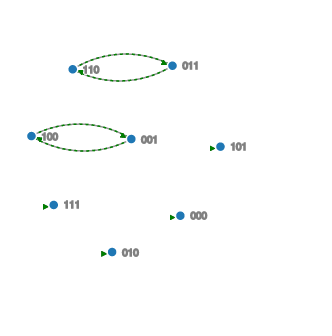
\includegraphics[width=0.79\textwidth]{network1.png}
  \label{fig:1}
  \caption{The network for the memories given in class.}
\end{figure}

\begin{figure}[h!]
 \centering
  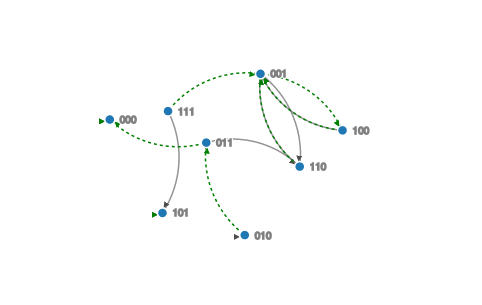
\includegraphics[width=0.79\textwidth]{network2.png}
  \label{fig:2}
  \caption{The network for the memories given in class, with a slight change so that the two memories are not symmetric. More interesting!}
\end{figure}

\begin{figure}[h!]
 \centering
  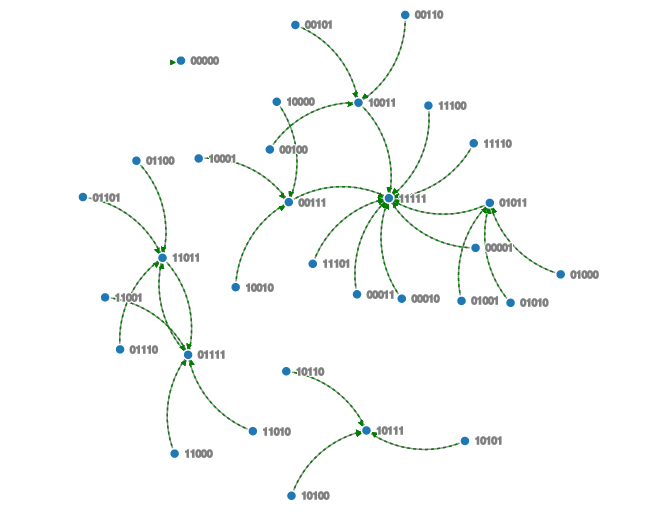
\includegraphics[width=0.79\textwidth]{network3.png}
  \label{fig:2}
  \caption{A bigger network having some trouble remembering things. Maybe I coded it wrong...}
\end{figure}

\clearpage
\pagebreak

\section*{Full code}

\lstinputlisting[]{bam_andy_driver.m}

\clearpage
\pagebreak

\lstinputlisting[language=Java]{js/bam.js}

\end{document}
